\documentclass[journal]{IEEEtran}
\input{settings}
\begin{document}

\section{提案モデル}
この章では、\ref{sec:ProposedModel-TemporalLogic}章で述べた記述法の応用例として、キャッシュを実装したウェブセキュリティモデルを提案する。

本研究では基礎モデルで包括されていないウェブの要素としてキャッシュに注目する。
\ref{sec:introduction}章に述べた通りキャッシュを利用する攻撃が数多く存在しており、また、キャッシュは一般的なユーザにも利用されるウェブの構成要素である。
したがって、キャッシュに関連した脆弱性はウェブの利用者に多大な影響を与えるため、ウェブの安全性を解析する上で不可欠な要素である。

\subsection{提案モデルの包括内容}
\label{sec:ProposedModel-Content}
提案モデルは基礎モデルを基に作成する。
基礎モデルからの変更点を以下に述べる。

\subsubsection{キャッシュ}
キャッシュはクライアント、サーバ、中継者のいずれかに属し、「格納と削除」、「再利用」、「検証」という三つの基本動作が可能である。
また、これらのキャッシュの動作はヘッダによって制御される。

\subsubsection{中継者}
中継者はクライアントやサーバとは異なるHTTPを構成する第三の要素であり、クライアントとサーバの通信経路上に存在する。
HTTP/1.1において、中継者は「プロキシ」、「ゲートウェイ」、「トンネル」の三種類が存在するが、これらのうちトンネルのみキャッシュを搭載しない。
したがって、キャッシュに注目する本提案モデルではプロキシとゲートウェイのみを包括する。

まず、中継者は独自にリクエストやレスポンスを生成することはなく、取得したリクエストやレスポンスの回送のみを行う。
しかし、キャッシュを用いた場合にのみ、リクエストをサーバに回送しレスポンスを得ることなく、キャッシュの再利用をもってリクエストに応答することができる。
また、プロキシとゲートウェイはその通信内容の編集が可能である。

\subsubsection{HTTPヘッダ}
基礎モデルに含まれるヘッダではキャッシュの動作の表現に不十分であるため、表\ref{tb:ProposedModel-Headers}に挙げるヘッダを新たに追加する。

\begin{table}[htb]
\centering
\caption{提案モデルで新たに包括するヘッダ}
\label{tb:ProposedModel-Headers}
\begin{tabular}{ll}
\hline
ヘッダ名 & 目的 \\
\hline
if-modified-since & 条件付きリクエストに使用 \\
if-none-match & 条件付きリクエストに使用 \\
etag & レスポンス内のコンテンツの固有値 \\
last-modified & レスポンス内のコンテンツの最終更新日 \\
age & レスポンスの経過時間 \\
cache-control & キャッシュの動作全般を制御 \\
date & レスポンスの生成時刻 \\
expire & レスポンスの有効期限 \\
\hline
\end{tabular}
\end{table}

また、表\ref{tb:ProposedModel-Headers}内のcache-controlヘッダはオプションによってキャッシュの動作を指定するため、そのオプションを付加可能とする。
利用可能なオプションを表\ref{tb:CacheControlOption}に挙げる。

\begin{table}[htb]
\centering
\caption{利用可能なcache-controlヘッダのオプション}
\label{tb:CacheControlOption}
\begin{tabular}{ll}
\hline
オプション名 & 用途 \\
\hline
max-age & レスポンスの有効期限を設定 \\
smax-age & 共有キャッシュでの有効期限を設定(最優先) \\
no-cache & 検証無しに再利用できない \\
no-store & そのレスポンスを格納を禁止 \\
no-transform & コンテンツの編集を禁止 \\
max-stale & 期限切れである場合に許容できる時間 \\
min-fresh & 有効期限まで最低残り時間 \\
only-if-cached & キャッシュの再利用でのみ応答 \\
must-revalidate & 有効期限切れの場合、検証無しに再利用できない \\
proxy-revalidate & must-revalidateと同じ(個人キャッシュ以外) \\
public & 共有キャッシュに格納してよい \\
private & 個人キャッシュに格納してよい \\
\hline
\end{tabular}
\end{table}

これら表\ref{tb:ProposedModel-Headers},\ref{tb:ProposedModel-Headers}の各項目のふるまいはHTTP/1.1の仕様に準拠する。

\subsubsection{ブラウザ}
基礎モデルでは表現の単純化のため、「ブラウザのメモリ領域は書き込みのみ可能」という制限がある。
しかし、この制限下ではキャッシュ内の格納レスポンスの削除や検証といった動作を実行することができず、キャッシュの動作を十分に表現することができない。
本研究で提案する時相論理の記述法を用いることでレスポンスの削除といった動作は容易に表現できるため、提案モデルではこの制限を取り除く。

\subsubsection{脅威モデル}
提案モデルの脅威モデルは基礎モデルのものを継承している。
すなわち、三種類の攻撃者とユーザのふるまいを脅威モデルとして設定し、攻撃者にキャッシュと中継者に関する攻撃の能力を新たに付与する。
以下に、三種類の攻撃者それぞれに付与する能力を示す。

\begin{itemize}
\item Web Attackerは複数の中継者を所有することができる。
しかし、その通信内容の編集や通信の遮断をすることはできず、内容をそのままに回送することのみ可能とする。
ただし、暗号化されていない場合、その通信内容を盗聴することは可能とする。
また、保有するクライアント、サーバ、中継者にキャッシュを搭載し、仕様通りに運用できる。
\item Network Attackerは上記のWeb Attackerの能力を全て持つ。
これに加えて、中継者を用いた暗号化されていない通信内容の改ざんと、通信の遮断は可能とする。
\item Gadget Attackerは中継者とキャッシュに関する能力は上記のNetwork Attackerと同様の能力を持つ。
\end{itemize}

\subsubsection{安全性要件}
基礎モデルには二つの安全性要件が設定されており、これらの変更はない。
ただし、Security Invariantsにおける「ウェブの各構成要素の仕様を侵さない」という文言にキャッシュや中継者の仕様を含む。

\subsection{キャッシュの作成}
\label{sec:CacheClass}
キャッシュを表すクラスをCode\ref{code:CacheClass}のように記述する。
抽象クラスとしてCacheクラスを定義し、個人キャッシュを表すPrivateCacheクラス、共有キャッシュを表すPublicCacheクラスを定義する。
また、CacheクラスにはCode\ref{code:LimitedCacheClass}に記述する制限を付与する。
付与される制限は以下の二点である。
\begin{itemize}
\item どのネットワーク上の端末にも属さないキャッシュは存在しない
\item 個人キャッシュはクライアントに属する
\item 共有キャッシュはサーバ、もしくは中継者に属する
\end{itemize}

\begin{lstlisting}[caption=Cacheクラス, label=code:CacheClass]
abstract sig Cache{}
sig PrivateCache extends Cache{}
sig PublicCache extends Cache{}
\end{lstlisting}

また、キャッシュを搭載するため、Code\ref{code:EndPoint}のように、構成要素のクラスを変更する。
HTTPにおけるクライアント、サーバ、中継者を包括するHTTPConfirmistクラスにCacheクラスを追加する。
また、このとき各端末は多くとも一台のキャッシュしか保有することができないものとする。
\begin{lstlisting}[caption=HTTPを利用するウェブの構成要素, label=code:EndPoint]
abstract sig HTTPConformist extends NetworkEndpoint{
	cache : lone Cache
}
\end{lstlisting}

\subsection{キャッシュの状態を表現するクラス}
\label{sec:CacheState}
Code\ref{code:CacheStateClass}のように、時間軸上の各時点におけるキャッシュの状態を表現するCacheStateクラスを作成する。
このCacheStateクラスはStateクラスを継承し、作成した時相論理に関する述語を利用可能な形式とする。
ここで、Stateクラスで定義した「不変項目」はCode\ref{code:CacheClass}で定義したCacheクラス、「変化項目」は格納レスポンスを表現するためのレスポンスの有限集合とする。
これに従い、不変項目を表すCacheEqItem、変化項目を表すCacheDifItemをCode\ref{code:CacheStateClass}に定義する。

また、Code\ref{code:CacheStateClass}では省略しているが、CacheStateには以下の制限を付与する。
これは、レスポンスがキャッシュに格納される場合に満たされなければならないの条件であり、HTTP/1.1の仕様に従っている。
\begin{itemize}
\item 個人キャッシュに格納されている場合、cache-controlヘッダのmax-ageオプション、もしくはdateヘッダとexpireヘッダが一つ含まれる
\item 共有キャッシュに格納されている場合、cache-controlヘッダのmax-ageオプション、s-maxageオプション、dateヘッダとexpireヘッダのいずれかが一つ含まれる
\item キャッシュに格納されている場合、必ずageヘッダが一つ含まれる
\end{itemize}

\begin{lstlisting}[caption=キャッシュの状態を表すクラス, label=code:CacheStateClass]
sig CacheState extends State{}{
	eq in CacheEqItem
	dif in CacheDifItem

	...
}
sig CacheEqItem extends EqItem{cache: one Cache}
sig CacheDifItem extends DifItem{store: set HTTPResponse}
\end{lstlisting}

また、これらの他に以下の制限を加える。
これらの制限は直接的に解析結果に影響するものではないが、可能な限りインスタンスの数を減らし解析を容易にするための工夫である。

\begin{itemize}
\item 同一内容のStateのインスタンスが複数存在しない。異なる時刻で同じ状態を取る場合には同じStateクラスに統合される
\item キャッシュが搭載されている端末が通信を行った場合に、そのキャッシュの状態が必ずインスタンスとして表現される
\item キャッシュに格納されている場合、必ずageヘッダが一つ含まれる
\end{itemize}

\subsection{キャッシュの動作}
\ref{sec:CacheClass}節で定義したCacheStateクラスを用いて、\ref{sec:ProposedModel-Content}節で述べたキャッシュの基本的な3つの動作をAlloyで表現する。

\subsubsection{レスポンスの格納と削除}
提案モデルにおいて、キャッシュにおけるレスポンスの格納と削除は以下のように動作するものとする。

\begin{itembox}[l]{レスポンスの格納}
キャッシュは、そのキャッシュが存在する端末が送受信したレスポンスを格納できる。
そのタイミングは、格納レスポンスを送受信したタイミングとする。
また、格納レスポンスは格納することのできる条件をすべて満たしているものとする。
\end{itembox}

\begin{itembox}[l]{レスポンスの削除}
キャッシュは任意のタイミングで、格納されているレスポンスをキャッシュ内から削除できる。
\end{itembox}

上記で定めたレスポンスの格納と削除は図\ref{fig:ProposedModel-ResponseStoreDelete}のように、二状態間の状態変化として表現する。
まず、レスポンスの格納はレスポンス時のキャッシュの状態において、格納レスポンスにそのレスポンスを追加することで表現できる。
これは、図\ref{fig:ProposedModel-ResponseStoreDelete}内のCacheState0,1における状態変化にあたる。
CacheState0は変化項目としてCacheDifItem0を持ち、CacheState1はCacheDifItem1を持つ。
そして、CacheDifItem0は格納レスポンスの集合が空集合であり、CacheDifItem1は格納レスポンスの集合にResponse0を持つ。
これは、StateTransaction0におけるレスポンスがResponse0であり、レスポンス時にそれがCache0に格納されたことを表す。
また、レスポンスの削除は前状態における格納レスポンスの一部を次状態に引き継がないことで表現する。
これは、図\ref{fig:ProposedModel-ResponseStoreDelete}内のCacheState1と2における状態変化にあたる。
この場合、CacheState2は変化項目としてCacheDifItem0を持つため、上述の格納の場合と状態変化が逆になる。
つまり、CacheState1の時点でCache0が格納していたResponse0を、CacheState2の時点では削除していることを表している。

\begin{figure}[htb]
\centering
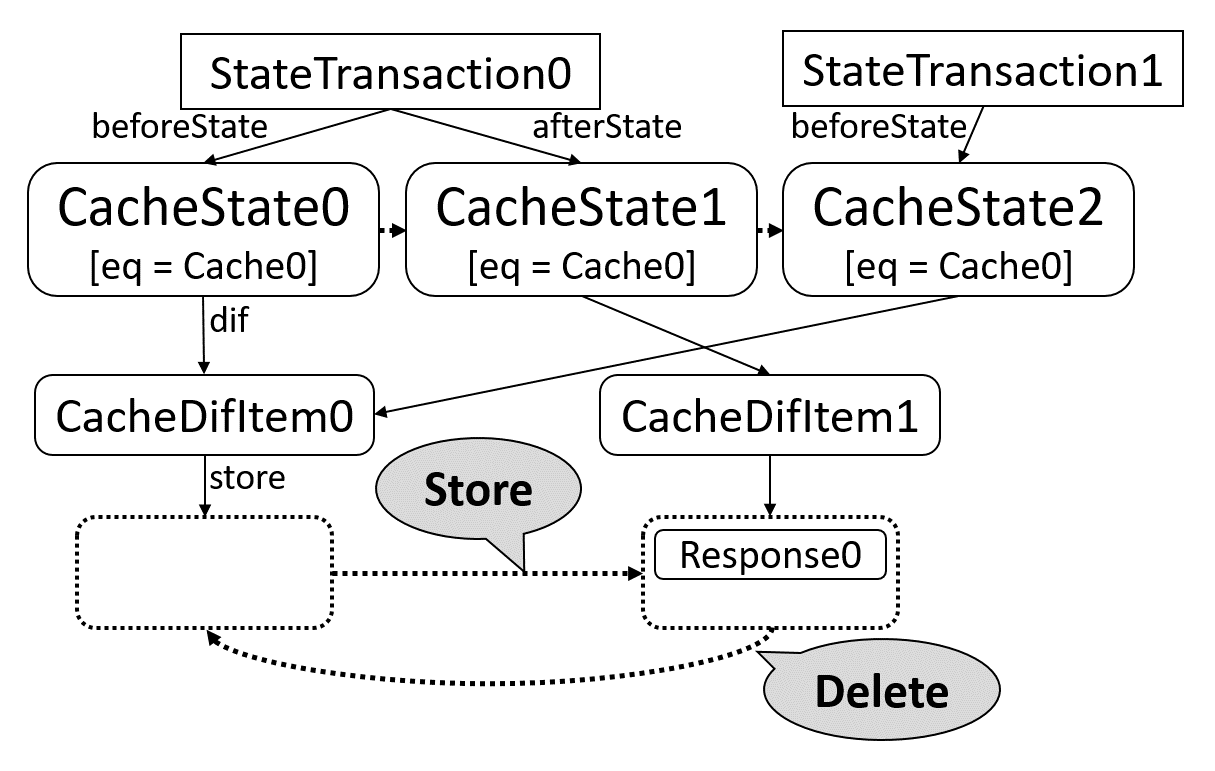
\includegraphics[width=\hsize]{./fig/ProposedModel-ResponseStoreDelete.eps}
\caption{キャッシュの格納と削除の表現}
\label{fig:ProposedModel-ResponseStoreDelete}
\end{figure}

また、以上の内容を提案モデルではCode\ref{code:StoreResponse}のように実装している。
すべてのCacheStateクラスのpostに対して、述語LastStateを用いて直前状態を取得し、それをpreとする。
ここでpostがリクエスト時の状態である場合、postの格納レスポンスの集合はpreの格納レスポンスの集合の補集合となる。
ここで、補集合とすることで前状態の格納レスポンスの一部がなくなることを容認し、格納レスポンスの削除を表現している。
また、postがレスポンス時の状態である場合、postの格納レスポンスの集合はpreの格納レスポンスの集合にpost時のレスポンスを加えた集合の補集合となる。
ここで、post時のレスポンスが集合に追加されることが、レスポンスの格納動作を表現している。

ただしこの記述のみでは各時点でのキャッシュの状態はその前状態に依存することになり、初期状態が無条件となる。
実際には、この場合の初期状態とはウェブ上における様々な通信が行われる前の状態を示すため、初期状態でキャッシュにレスポンスが格納されていることはない。
したがって、初期状態の格納レスポンスの集合を空集合とする制限を、述語InitailStateを用いて記述している。

\begin{lstlisting}[caption=レスポンスの格納と削除の表現, label=code:StoreResponse]
fact flowCacheState{
	all cs:CacheState |
		InitialState[cs] implies
			no cs.dif.store

	all pre, post:CacheState, str:StateTransaction |
		LastState[pre, post, str] implies {
			post in str.beforeState implies post.dif.store in pre.dif.store
			post in str.afterState implies post.dif.store in (pre.dif.store + str.response)
		}
}
\end{lstlisting}

\subsubsection{レスポンスの再利用}
提案モデルにおいて、キャッシュによるレスポンスの再利用は以下の動作を示す。

\begin{itembox}[l]{レスポンスの再利用}
キャッシュは、そのキャッシュが存在する端末が送受信するリクエストに対して、キャッシュ内の格納レスポンスで応答できる場合、そのレスポンスを用いて応答することができる。
ここで、リクエストの送信者が自身のキャッシュで再利用を行う場合、リクエストは実際はネットワーク上に発信されない。
\end{itembox}

上記で定めたレスポンスの再利用は、提案モデル内では本来発生するレスポンスの代わりとなって発生する。
したがって、既存モデルにおいてレスポンスを表すHTTPResponseクラスと同列に、CacheReuseクラスを定義する(Code\ref{code:CacheReuseClass}参照)。
HTTPResponseクラスはHTTPプロトコル上のイベントを表すHTTPEventクラスを継承しているため、CacheReuseクラスもHTTPEventクラスを継承する。
そして、CacheReuseクラスにある一つのレスポンスを関連付けることで、どのレスポンスを再利用したかを表現する。
また、HTTPEventクラスにおいて、どの端末からどの端末に対するイベントであるかは定義されており、これを利用することで再利用したレスポンスの送信元と送信先を表現する。
しかし、HTTPEventクラスでは送信元と送信先の他に、そのイベントに含まれるヘッダとボディが定義されている。
実際のレスポンスの再利用では、送信されるのは再利用するレスポンスのヘッダとボディであり、それは上記の再利用対象のレスポンスとの関連付けで表現されているためこの二項目は不必要である。
したがって、CacheReuseクラスとヘッダとボディの関係性は無視することができるが、ヘッダやボディを表すインスタンスは非常に多いため、無制限とした場合には無駄な計算時間を要することとなる。
このような要因から、CacheReuseクラスのヘッダとボディは空集合とし、計算時間の短縮を図る。

\begin{lstlisting}[caption=CacheReuseクラス, label=code:CacheReuseClass]
sig HTTPResponse extends HTTPEvent {
	statusCode: one Status
}
sig CacheReuse extends HTTPEvent{
	target: one HTTPResponse
}{
	no headers
	no body
}
\end{lstlisting}

上記で定義したCacheReuseクラスを用いて再利用を表現するため、CacheReuseイベントが発生する条件を、実際のキャッシュの動作に基づいて以下のように作成する。
\begin{itemize}
\item 再利用レスポンスの送信先は、その再利用を発生させたリクエストの送信元である
\item 再利用レスポンスの送信元は、その再利用を発生させたリクエストの送信元か送信先のいずれかである
\item 再利用を行うキャッシュの再利用直前の状態において、再利用するレスポンスが格納レスポンスに含まれている
\item 再利用するレスポンスと、その再利用を発生させたリクエストが表すURIが一致している
\end{itemize}

上記の条件の二点目において、再利用レスポンスの送信元がリクエストの送信元となる場合を認めるのは、そのリクエストを送信した端末のキャッシュによるレスポンスの再利用を想定するためである。

\subsubsection{格納レスポンスの検証}
\label{sec:CacheVerification}
提案モデルにおいて、キャッシュによる格納レスポンスの検証を以下のように定義する。

\begin{itembox}[l]{格納レスポンスの検証}
格納レスポンスは、格納レスポンスが再利用可能であるかを判定するために、条件付きリクエストを送信しオリジンサーバに問い合わせを行う。
条件付きリクエストは、if-modified-sinceヘッダかif-none-matchヘッダのいずれかが含まれるリクエストのことを指す。
これらのヘッダで送信される値を用いることで、オリジンサーバは格納レスポンスが最新のものと同一であるかを判定でき、再利用の可否をレスポンスで送信する。
検証が正常に終了した場合、このレスポンスの状態コードは304か200となる。
状態コードが304である場合は、そのヘッダやボディの値に関係なくキャッシュは格納レスポンスを再利用できる。
状態コードが200である場合は、格納レスポンスは再利用不可であり、このレスポンスをキャッシュに格納して再利用する。
また、検証後はどちらの場合も再利用可能なレスポンスの一つを除いて、同一のURIに対するレスポンスはキャッシュ内には存在しない。
\end{itembox}

この動作の実装は以下の二つを表現することで実現できる。
\begin{itemize}
\item レスポンスの再利用が行われている場合に、その再利用レスポンスが検証済みであるかを判定する述語
\item 条件付きリクエストに対するサーバの動作
\end{itemize}

まず、検証済みかを判定する述語checkVerificationをCode\ref{code:checkVerification}に示す。
この述語checkVerificationはStateTransaction(strとする)を入力とする。
述語checkVerificationは、strが再利用によって応答されているトランザクションであり、かつ、strのリクエストと再利用の間に条件付きリクエストを含むトランザクションが成立している場合に真となるように作成し、その論理は以下のように表せる。

\begin{itembox}[l]{述語checkVerification}
入力であるStateTransactionクラスのインスタンスstrが再利用を行っており、かつ、以下を満たすStateTranactionのクラスのインスタンスstr'が存在する場合に、本述語は真となる。
\begin{itemize}
\item strとstr'は異なるトランザクションである
\item str'のレスポンスが存在する。つまり、通信が正常に完了している
\item str'のリクエストはstrの後に発生し、str'のレスポンスはstrの再利用より前に発生している
\item str'のリクエストは、strの再利用が行われるキャッシュが属する端末から、再利用するレスポンスの送信元に送信されている
\item strとstr'での要求URIが同一である
\item 検証対象の格納レスポンスにetagヘッダかlast-modifiedヘッダが含まれている
\item 検証対象の格納レスポンスにetagヘッダが含まれている場合、str'のリクエストにif-none-matchヘッダが含まれる
\item 検証対象の格納レスポンスにlast-modifiedヘッダが含まれている場合、str'のリクエストにif-modified-sinceヘッダが含まれる
\end{itemize}
\end{itembox}

また、条件付きリクエストに関するサーバの動作をAlloy上で表現する。
HTTPTransactionクラスのインスタンスtrが条件付きリクエストを含む通信である場合、そのリクエストを受信したサーバは以下を満たすように条件を付加する。
\begin{itemize}
\item 検証後に、その検証対象のレスポンスのURIを持つ格納レスポンスは一つとなる
\item trのレスポンスの状態コードは200か304である
\item trのレスポンスの状態コードが200である場合、trのレスポンスはキャッシュに格納される
\item trのレスポンスの状態コードが304である場合、trのレスポンスはキャッシュに格納されない
\end{itemize}

\subsection{中継者の実装}
提案モデルにおいて中継者はHTTP/HTTPSプロトコルで動作し、プロキシとゲートウェイを包括する。
したがって、HTTPに遵守する端末を表すHTTPConfirmistを継承する形で中継者のクラスを宣言する。
また、中継者のクラスを継承し、プロキシとゲートウェイのクラスを宣言する。
これらのクラスは以下のコードで実装される。

\begin{lstlisting}[caption=中継者のクラス, label=code:IntermediaryClass]
abstract sig HTTPIntermediary extends HTTPConformist{}
sig HTTPProxy extends HTTPIntermediary{}
sig HTTPGateway extends HTTPIntermediary{}
\end{lstlisting}

また、この中継者の動作をAlloyで記述する。
中継者の動作はリクエストの送信先がHTTPIntermediaryであり、かつ、レスポンスが存在するHTTPTransactionに対する条件として記述できる。
このようなHTTPTransactionのインスタンスtrに対して、以下を満たすHTTPTransactionのインスタンスtr'が少なくとも一つ存在する。
\begin{itemize}
\item trとtr'は異なるトランザクションである
\item tr'のリクエストはtrのリクエストの後に発生し、tr'のレスポンスはtrのレスポンスの前に発生する
\item tr'のリクエストの送信元は、trのリクエストの送信先である中継者である
\item trとtr'のリクエストのURIは同一である
\item trとtr'のレスポンスのbodyと状態コードは同一である
\end{itemize}
ただし、上記の動作は正当なユーザに管理された中継者の動作であり、攻撃者が管理する中継者のふるまいはこの限りではない。

\end{document}
